%---------------------------------------------------------------------------

%---------------------------------------------------------------------------

\documentclass[11pt]{article}

\usepackage{vmargin}
% somewhat large on the page
\setmargins%
{.8in}{.5in}{500pt}{650pt}%  leftmarg   rightmarg textwidth  textheight
{25pt}{40pt}{0pt}{0pt}%    headheight headsep   footheight footskip


% loading Libs
\usepackage{graphicx}

\usepackage[backend=biber, style=alphabetic, sorting=ynt]{biblatex}

\addbibresource{./ref.bib}

\graphicspath{{./Images/}}


% some minor customization

\addtolength{\parskip}{1ex}
\setlength{\parindent}{0in}

\newcommand{\ignore}[1]{}
\newcommand{\remark}[1]{[{\small{\bf Editorial Remark: }#1}]}

%---------------------------------------------------------------------------
% now for the fun part

\begin{document}
	
\vspace*{-10mm}

\framebox{
\begin{minipage}[t]{6in}
\vspace{2ex}
 
{\LARGE\bf  Reproduction of A. Rahman paper Results }
\vspace{2ex}

Project : 2
\vspace{2ex} 

Name: Satyendra Pandey
\vspace{2ex} 

Roll No.: 14807611
\vspace{2ex} 

Course :  Molecular Dynamics and Simulations.
\vspace{1ex} 

\end{minipage}
}%% end framebox

\vspace{3ex}


%---------------------------------------------------------------------------

\section{Introduction}

In this project, We are goint to write a molecular dynamics code to simulate liquid argon atoms. \linebreak
We are also going to reproduce the results " {\bf Velocity autocorrelation and Radial pair distribution}" from classical paper of A. Rahman.

%\subsection{Test Subsection}
%---------------------------------------------------------------------------


\section{Molecular Simulation}

Molecular dynamics (MD) is a computer simulation method for studying the physical movements of atoms and molecules. The atoms and molecules are allowed to interact for a fixed period of time, giving a view of the dynamic evolution of the system. 

\subsection{Description of project}
In this project We have used 864 atoms of argon and arranged them in a cubical box with periodic box conditions as well as we make sure that two particles are atleast $\sigma$ distance awake from other molecules.

\subsection{Parameters Used}
%\begin{enumerate}
%\item iidij
%\item Here is the second step.
%\item Don't all algorithms have to have 3 steps?
%\end{enumerate}
Here is the list of parameters used in MD simulations :
\begin{itemize}
\item $\sigma$ = 3.4
\item R-cutoff = 7.65
\item num-of-particles = 864
\item mass = $6.69 * {10^{-26}}$ Kg
\item kb = $1.38 * {10^{-23}}$ J/K
\item Temp = 94.4 K
\item box size = 34.778 A
\item Density = $1.374 \hspace{.2cm} gm/cm^3$
\end{itemize}

\subsection{Algorithms Used In code}
Here is some of the key steps taken to Write a Optimised Algo for MD Simulation.
\begin{description}
\item[Random velocity and position Allocation]: \newline
To Generate Random velocity and position I have used {\bf Numpy} module in python which can give use normnal distribution by providing mean and standard deviation of the distribution. \\
I used linespace to create a solid cubic lattice and then removed atoms from different positions.\\
For velocity I have given values of sigma and mean such that It gives us a distribution with temperature as much needed.

\item[Algorithm For periodic Boundry condition]: \\
 Here is code from force and potential calculation of Periodic box condition \\
 
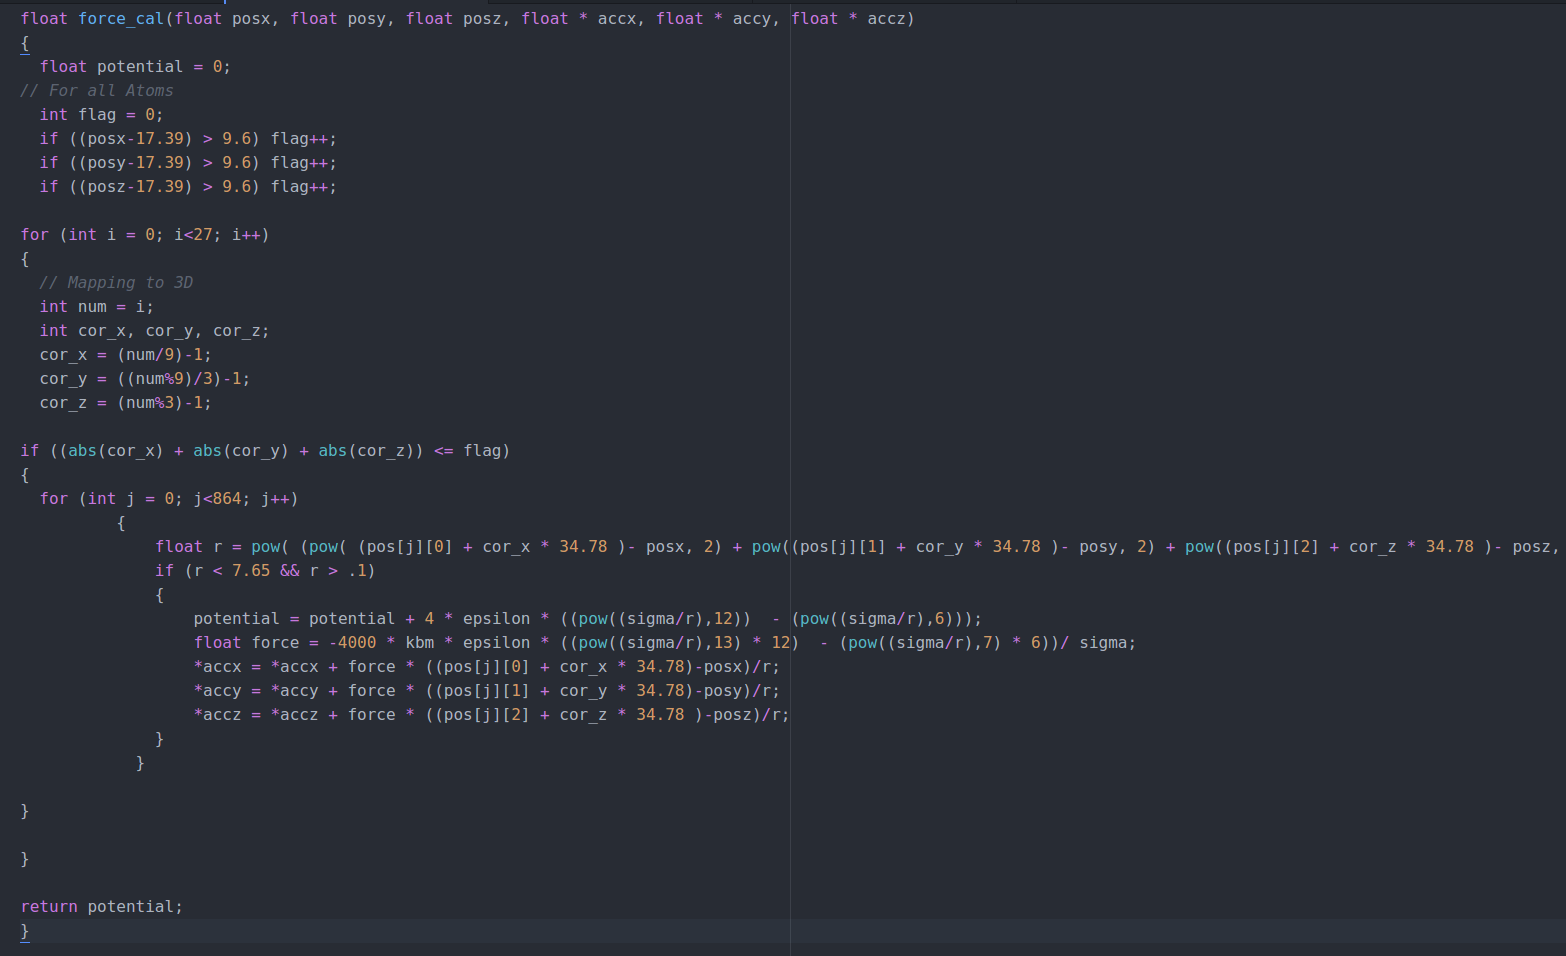
\includegraphics[width=18cm,height=14cm,angle=0]{Algo}

\hspace{2cm}
 
Algo in above Image reduce Running time significantly by Skipping irrelevent scenarios.\\
 
\item[Velocity verlet Algorithm]: \\ 
\vspace{.1cm}\\
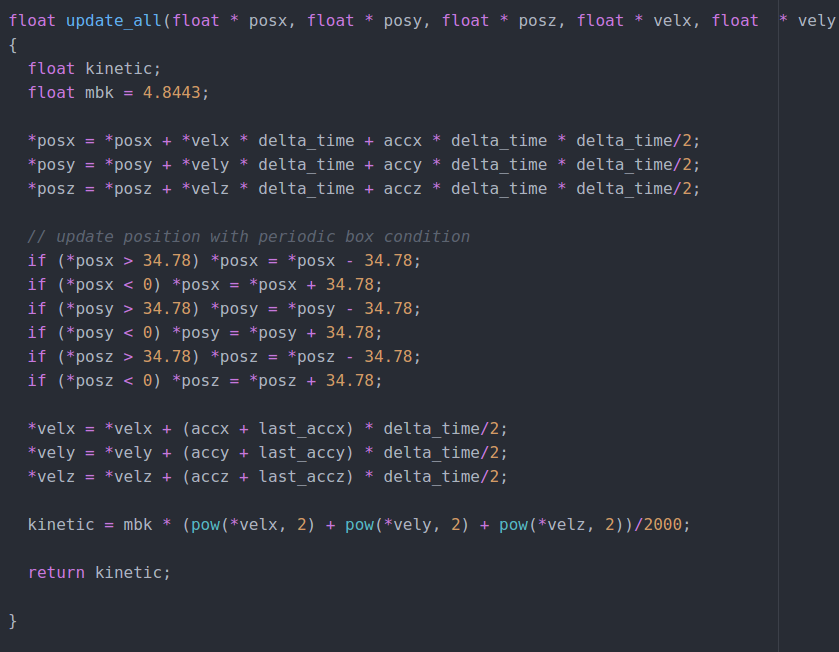
\includegraphics[width=17cm,height=8cm,angle=0]{update}
 
\end{description}

\section{Formula used}

\begin{itemize}
	\item \textbf{Leonard-Jones potential :} \\
	\vspace{.1cm}\\
	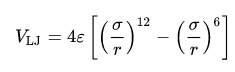
\includegraphics[scale=.7]{lj}
	\vspace{.1cm}
	\item \textbf{Radial pair Distribution :} \\
	\vspace{.1cm} \\
	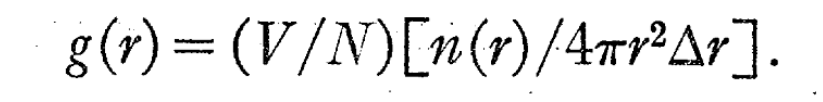
\includegraphics[scale=.275]{Rad} 
	\vspace{.1cm}
	\item \textbf{Temperature calculation :} \\
	\vspace{.1cm} \\
	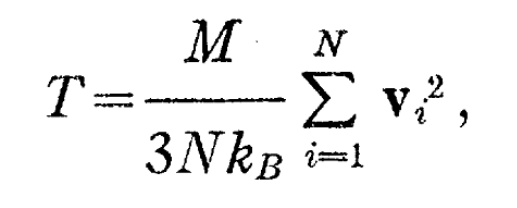
\includegraphics[scale=.275]{temp} 
	\vspace{.1cm}
	\item \textbf{Velocity auto-correlation :} \\
	\vspace{.1cm} \\
 	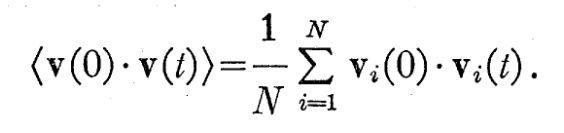
\includegraphics[scale=.35]{vel}
	\vspace{.1cm}
	
\end{itemize}

%---------------------------------------------------------------------------
\newpage

\section{Results}

\vspace{.5cm}

\subsection{Velocity Autocorrelation : }

Velocity autocorrelation is a tool to measure diffusion coefficient in MD simulations. \\
In velocity correlation we take velocity at a time t0 and we measure correlation of velocity withy time. \\
We get negative value of velocity correlation after sometime which generally comes due to back scatering of atoms, Also after long time all correlation fades away and it tends to zero.\\

In this experiment I have taken t0 as t = 0, I have moniterd it till t = 5 pico seconds. We can see that my plots qualitatively matches with Rahmans paper but in Rahmans paper it comes to zero at nearly .5 Pico seconds but in my simulation it comes to zero around .75 seconds.\\


\vspace{.2cm}


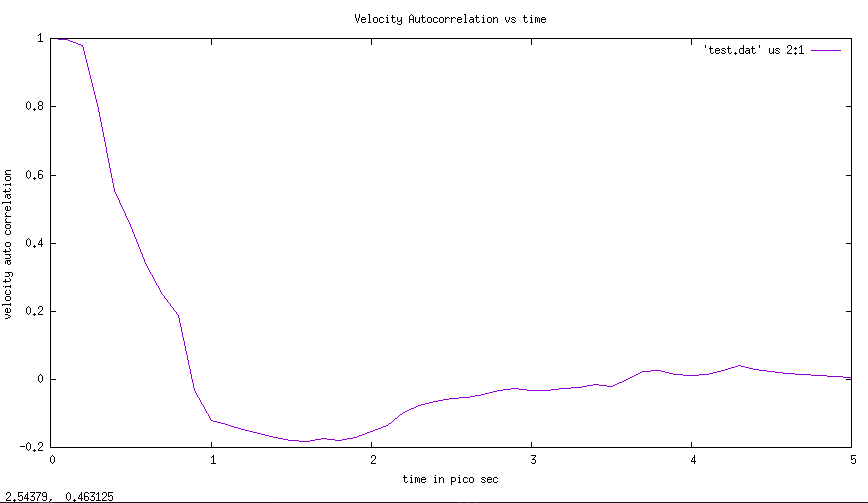
\includegraphics[width=18cm,height=12cm,angle=0]{Velo_autocor}

\vspace{.7cm}

Above picture shows Velocity auto-correlation with time.

\subsection{Radial Pair Distribution : }

\vspace{.2cm}

Radial Pair Distribution is a tool of molecular dynamics which describes how density varies as a function of distance from a reference particle. It can also be used to study phage-change behaviour of a material.\\

In this experiment I have taken delta-r as 0.8 A. \\
To calculate radial pair distribution I have taken an atom randomly and find the radial distribution surrounding that atom. We can see that In Rahmans paper, we can see the first peak at 3.7 A and in my simulation results it coming to be around 4A "{\it there is a peak near 3.7 too.}" Also we can see that second peak in rahman's paper is around 7A but in my simulations it's around 6A. it matches with rahman paper's results qualitatively with some error in quantative data.


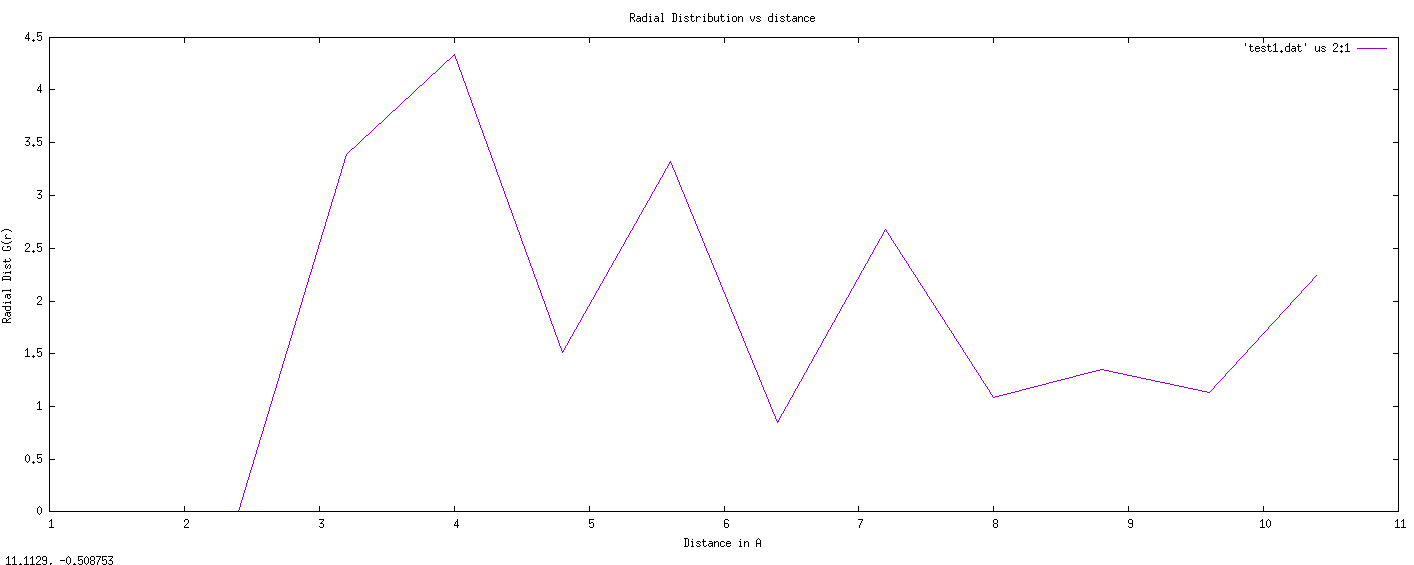
\includegraphics[scale=.367]{Radial}


\vspace{.4cm}


Above picture shows radial distribution function.

\vspace{.7cm}



\begin{thebibliography}{9}
	\bibitem{latexcompanion} 
	 A. Rahman,  Physical Rev.136,  A405 (196) 
	 Motion of Atoms in Liquid Argon
	 \\\texttt{http://theo.ism.u-bordeaux.fr/J-C.Soetens/doc/4TCH914U/Rahman\_PhysRev\_1964.pdf}
	
	
	\bibitem{einstein} 
	Molecular Modeling by A. R.Leach \\
	
	\bibitem{einstein} 
	Understanding Molecular Simulation by Frenkel and Smith

\end{thebibliography}




\end{document}